\section{Complementary Analysis Targeting Low Signal Masses}
\label{sec:ewk:LM}

The analysis discussed in this chapter is limited in sensitivity for low \mhino, as it is clear from Figure \ref{fig:exclusion_high}. 
This is because when \mhino approaches the Higgs mass, the decay products (Higgs boson and \gravino)
have increasingly low \pt, and a low \pt \gravino does not produce enough \met to fire the \met trigger and be selected 
in the analysis. 
To gain sensitivity also to the low-\mhino part of the mass spectrum, which is particularly interesting for Naturalness arguments, 
this analysis is complemented by a second analysis that targets low-\met events, referred to as "low-mass" analysis. 



\section{Combined Results}

\begin{figure}[htbp]
	\centering
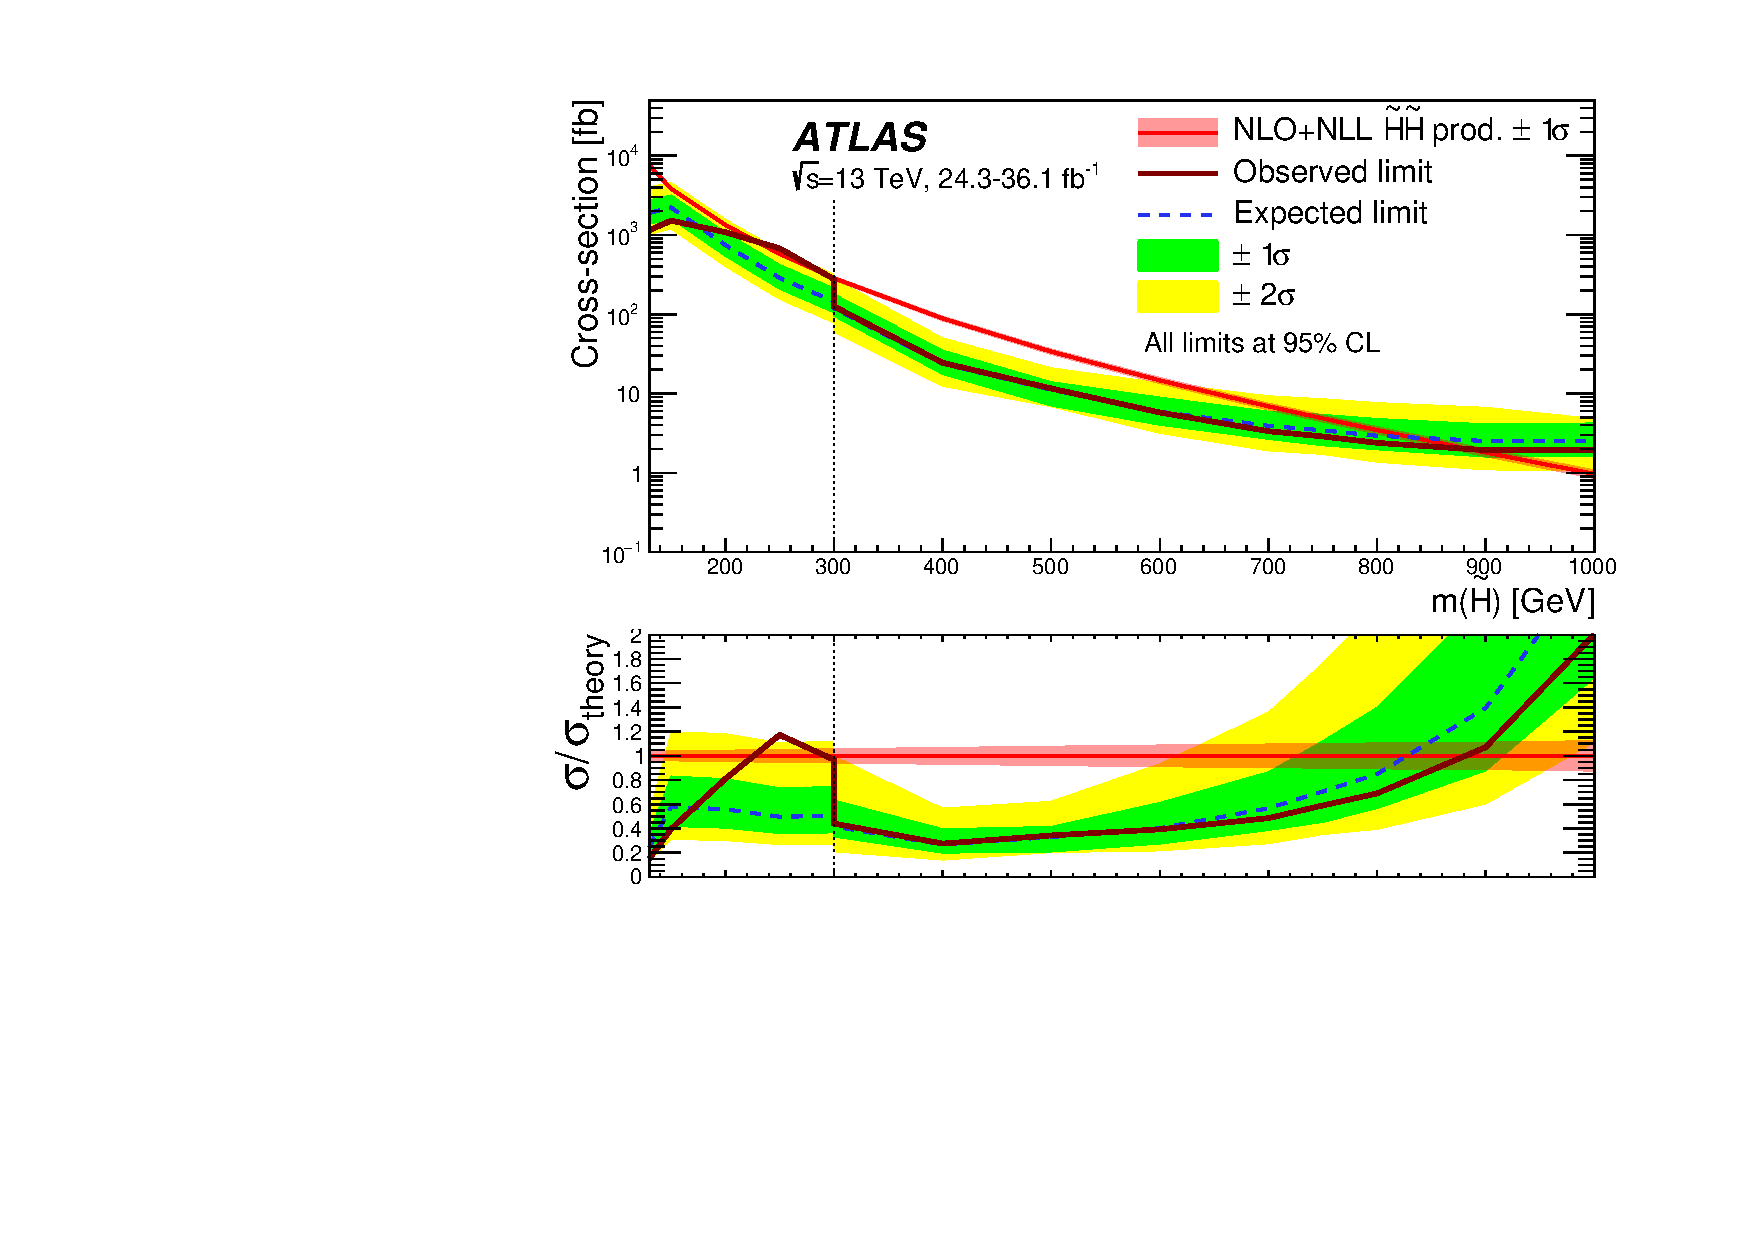
\includegraphics[width=0.75\textwidth]{figures/ewk_prod/interpretation/GGMupperLimit_unblinded_jump}
	\caption{The observed (solid) vs expected (dashed) 95\% upper limits on the \hino\ pair production cross-section as a function of \mhino.  The 1$\sigma$ and 2$\sigma$ uncertainty bands on the expected limit are shown as green and yellow, respectively. The theory cross-section and its uncertainty are shown in the solid and shaded red curve.
   The results of the low-mass analysis are used below $\mhino = 300$ GeV, while those of the high-mass analysis are used above. 
   Figure from Ref \cite{Aaboud:2018htj}. } 
	\label{fig:exclusion}
\end{figure}


\begin{figure}[htbp]    
	\centering    
    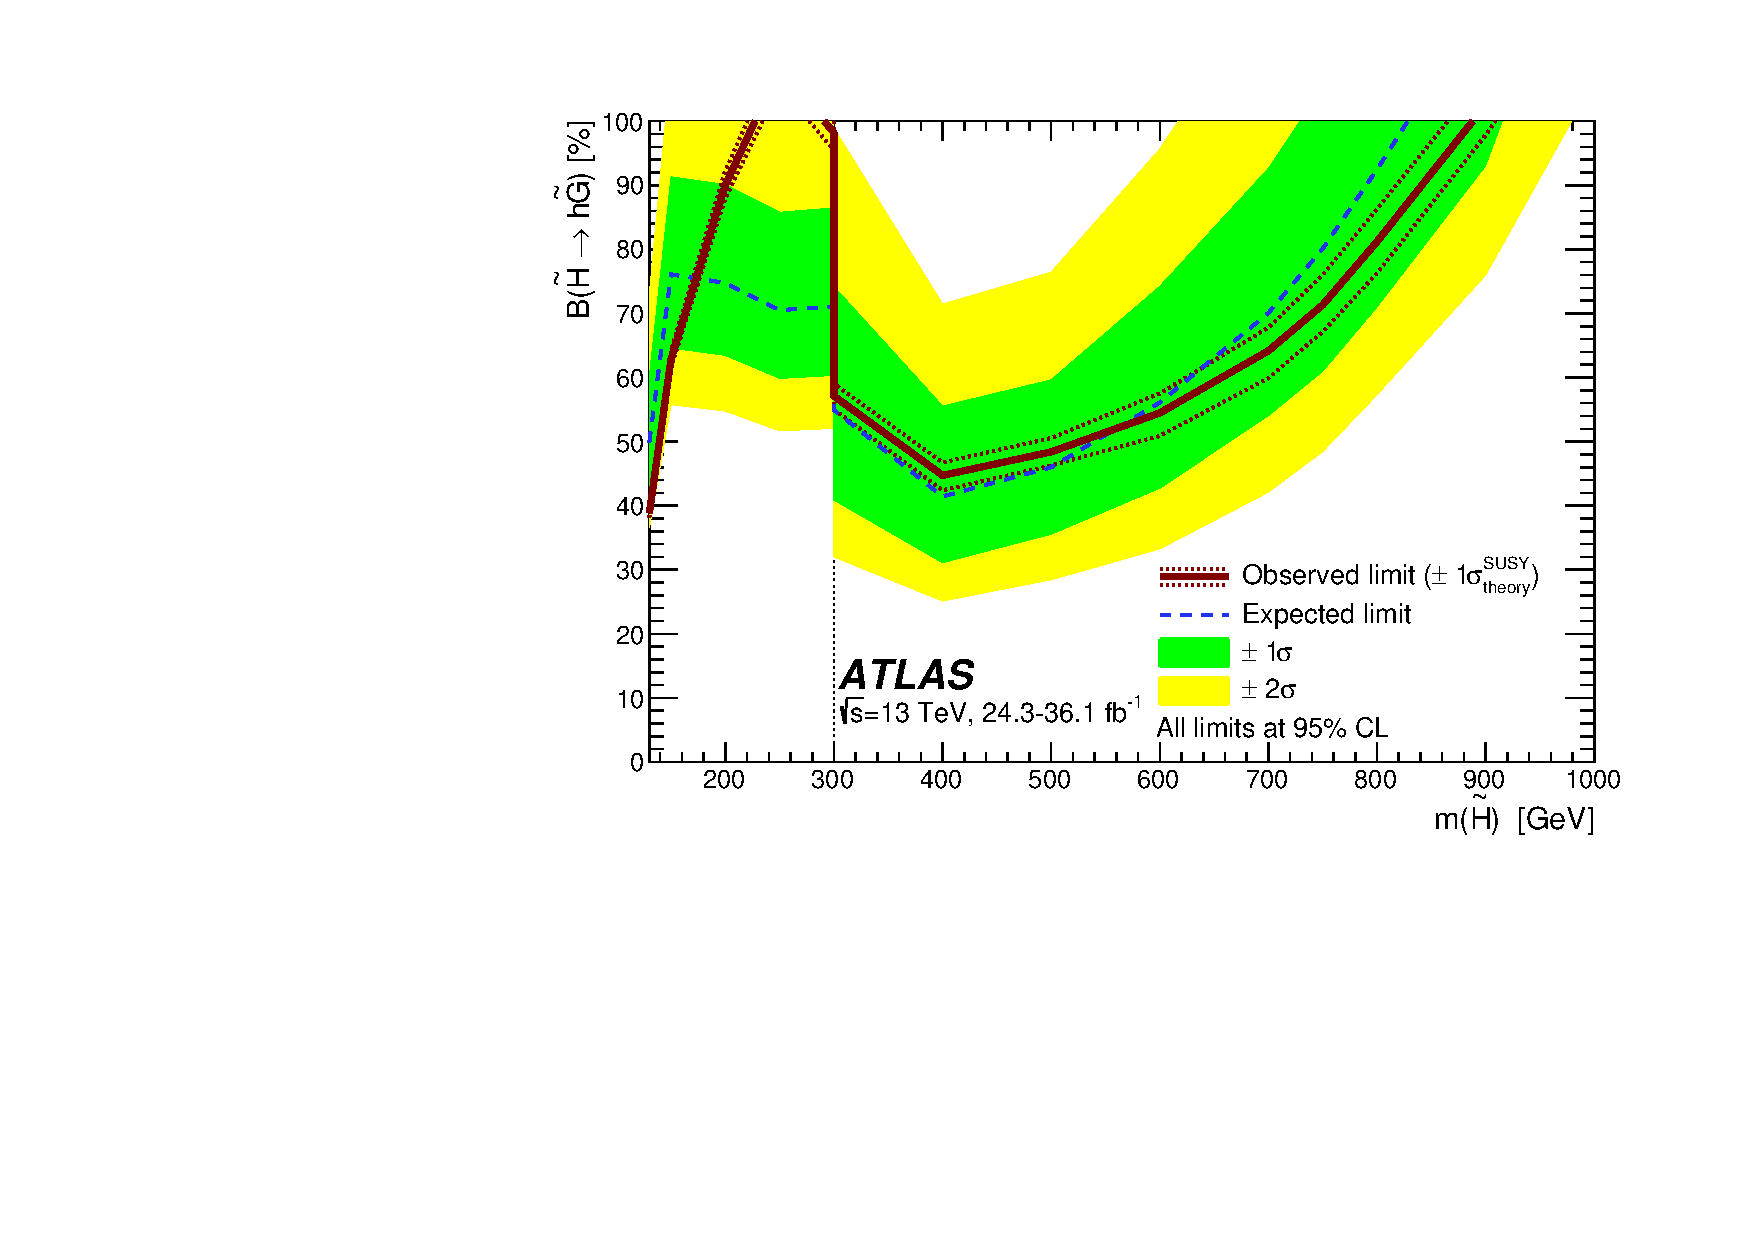
\includegraphics[width=0.75\textwidth]{figures/ewk_prod/interpretation/my_br_plot_unblind_yellow_band}\label{fig:exclusion_br}
	\caption{The observed (solid) vs expected (dashed) 95\% limits in the \mhino\ vs $B(\hino\rightarrow h \tilde{G})$ plane, where $B(\hino\rightarrow h \tilde{G})$ denotes the branching ratio for the decay $\hino \rightarrow h \gravino$. The 1$\sigma$ uncertainty band is overlaid in green and the 2$\sigma$ in yellow.
	The results of the low-mass analysis are used below $\mhino = 300$ GeV, while those of the high-mass analysis are used above.
	 The regions above the lines are excluded by the analyses. Figure from Ref \cite{Aaboud:2018htj}. } 
	\label{fig:exclusion}
\end{figure}


